\chapter{Spezifikation der funktionellen Anforderungen}
\section{Produktbeschreibung}
TODO: Blablabla, alles wichtig und ganz toll

\section{Funktionelle Anforderungen}
\subsection{Umgebungsmodell}

\subsubsection{Ereignistabelle}
%wenn die Tabellen zu lang werden -> longtable

\begin{tabular}[ht]{|l|l|l|l|}
\hline
Nr & Ereignis & Datenfluß im System & Antwort des Systems \\
\hline\hline
1. & Administrator: & Benutzerdaten & Best\"atigung\_Benutzer\"anderung \\
   & erg\"anzt Benutzer& & \\
   & ver\"andert Benutzer& & \\	
   & l\"oscht Benutzer& & \\	
\hline
2. & Benutzer: & Literaturdaten & Best\"atigung\_Literatur\"anderung \\
   & erg\"anzt Literatur & &  \\
   & ver\"andert Literatur & &  \\
   & l\"oscht Literatur & &  \\
\hline
3. & Benutzer: & Kommentardaten & Best\"atigung\_Kommentar\"anderung \\
   & erg\"anzt Kommentar & & \\
   & ver\"andert Kommentar & &\\
   & l\"oscht Kommentar & & \\
\hline
4. & Gast sucht Literatur& Suchbegriff & Suchergebnis \\
\hline
5. & Gast w\"ahlt Literatur & Literaturnummer & Literaturdaten \& Kommentare \\
\hline
6. & Gast exportiert Literatur & Exportanfrage & Literaturdaten in BibTex \\
\hline
\end{tabular}

\subsubsection{Kontextdiagramm}

%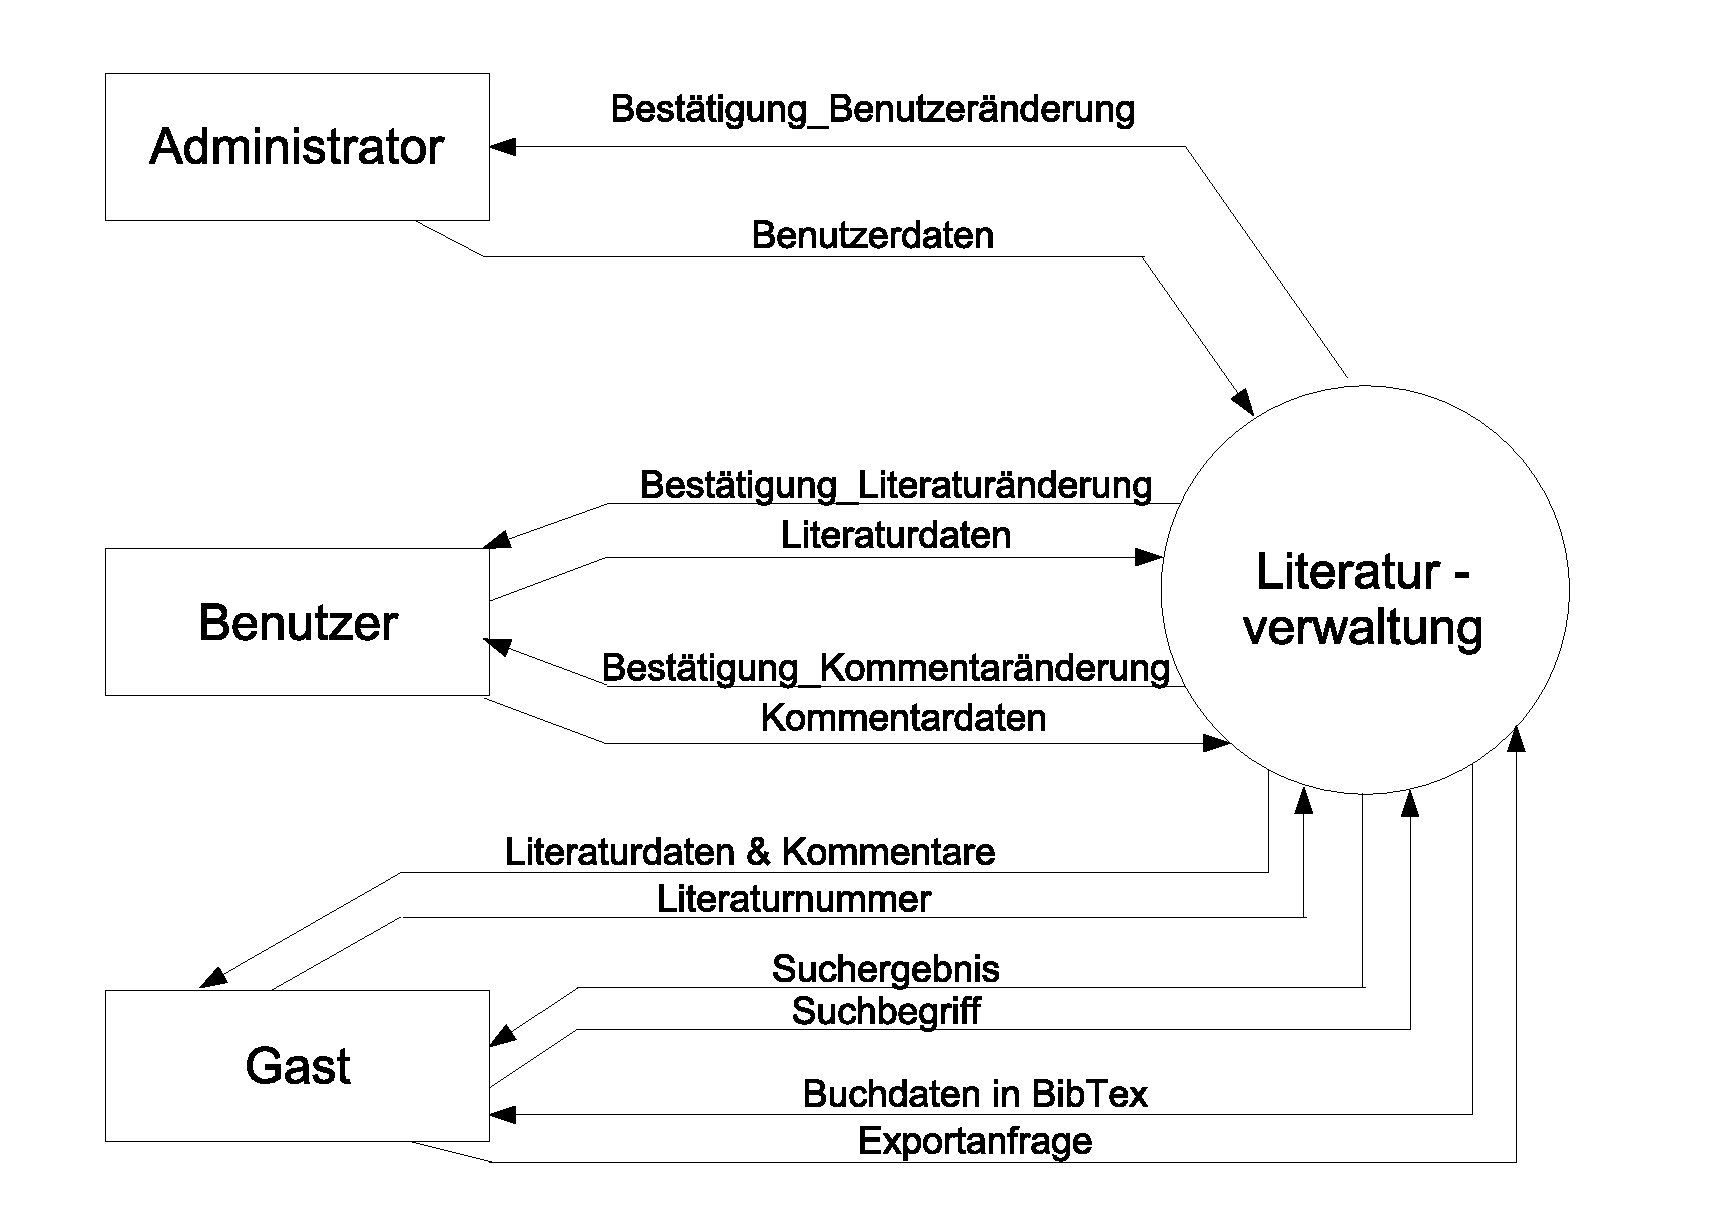
\includegraphics[scale=0.5]{kontextdiagramm}
\centerline{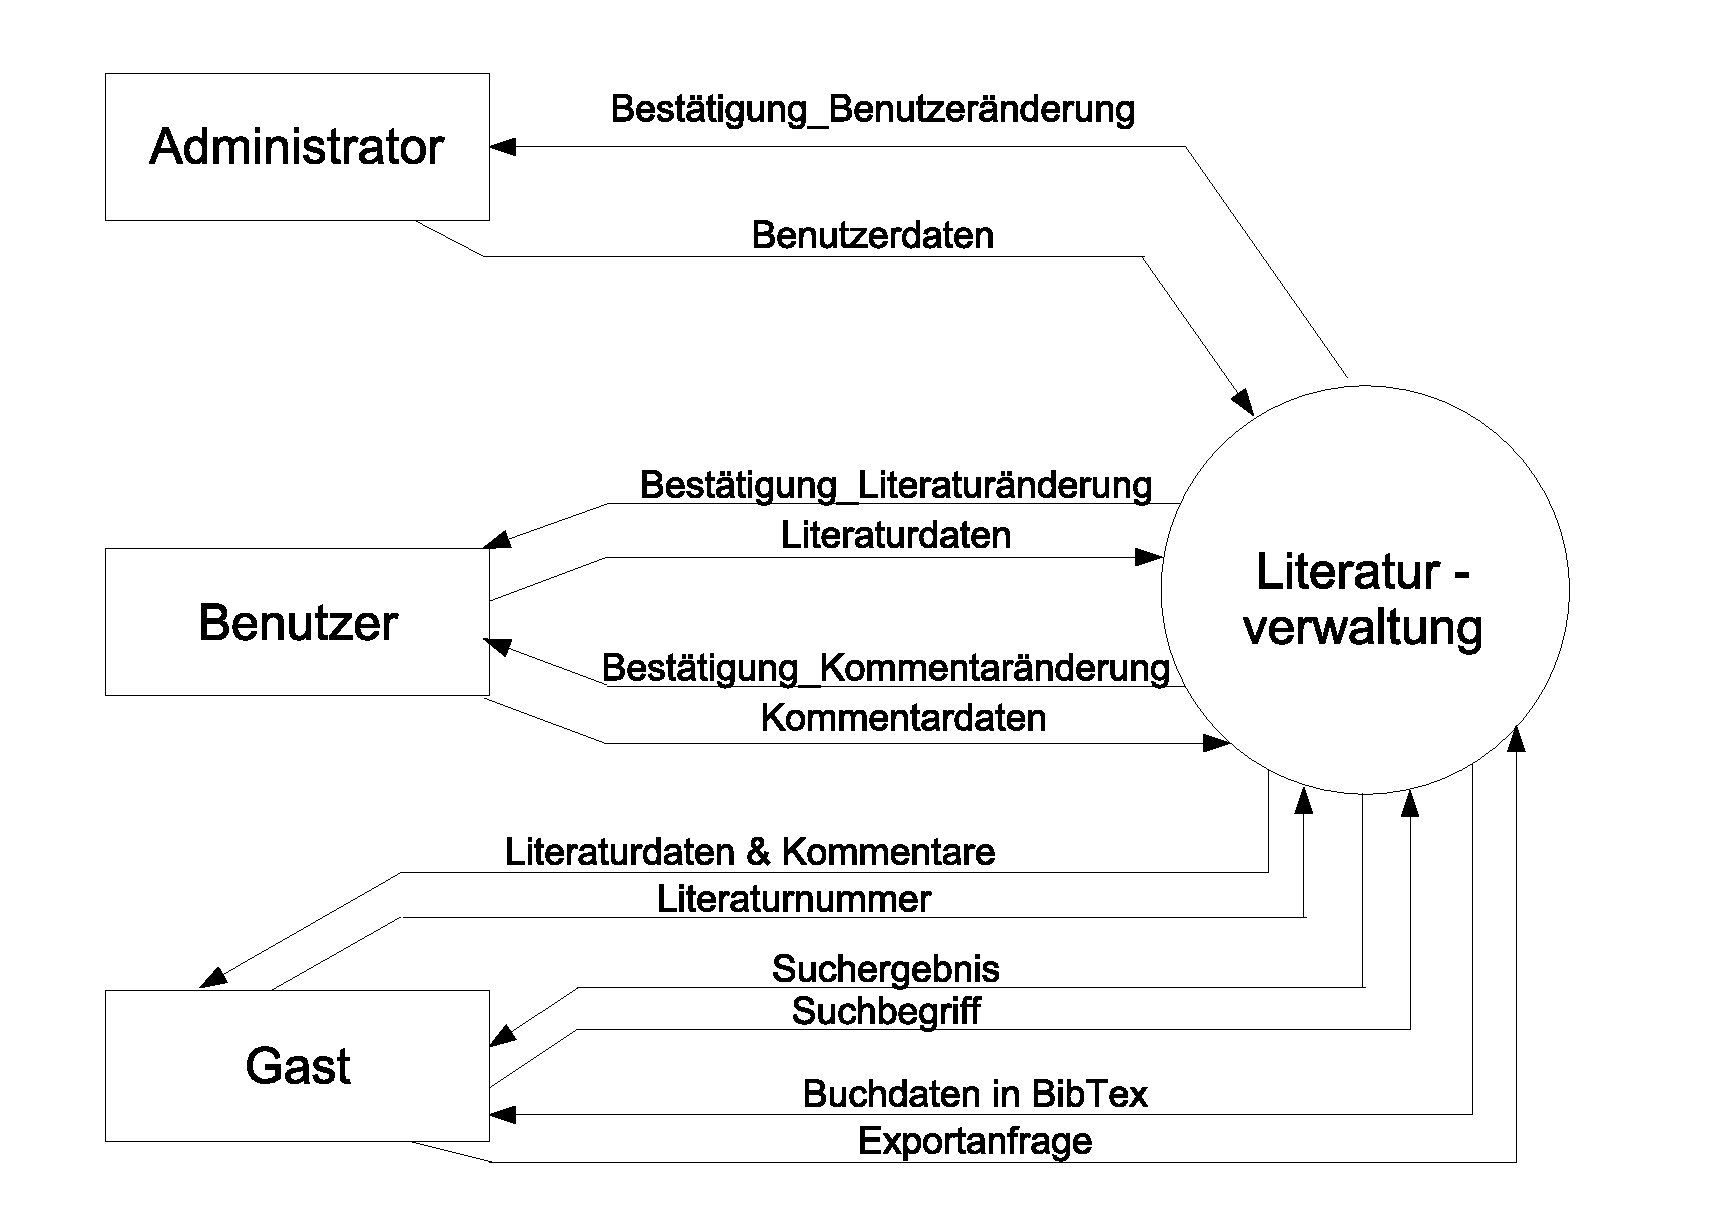
\includegraphics[scale=0.5]{kontextdiagramm}}

\subsection{Verhaltensmodell}
\subsubsection{Grobes Verhaltensmodell (vergröbertes primäres Verhaltensmodell)}
TODO
%\includegraphics[scale=0.5]{verhaltensmodell_grob}

\subsubsection{Primäres Verhaltensmodell}
\paragraph{Teilmodell blabla}
TODO
%\includegraphics[scale=0.5]{erhaltensmodell_blabla}

\paragraph{Teilmodell bloblo}
TODO
%\includegraphics[scale=0.5]{verhaltensmodell_bloblo}

\subsubsection{Verfeinerungen der Prozesse des primären Verhaltensmodells}
\paragraph{Verfeinerung zum Prozess: ieeekks}
TODO
%\includegraphics[scale=0.5]{prozess_ieeekks}

\paragraph{Verfeinerung zum Prozess: arrgghhh}
TODO
%\includegraphics[scale=0.5]{prozess_arrgghhh}

\subsubsection{Datenkatalog}
\begin{tabular}[ht]{|l|l|}
\hline
Element & Strukturbeschreibung \\
\hline\hline
% Mitglieder
\emph{Benutzer} & \{Benutzer\} \\
\hline
Benutzer  & @Benutzer\_Nr + Name + Login + Passwort + Rechte \\
\hline
Benutzer\_Nr & gZahl *6stellig, 000001 $\leq$ Benutzer\_Nr $\leq$ 999999* \\ 
\hline
Name & <Vor>Name + <Nach>Name \\
\hline
Login & Zeichenkette12 \\
\hline
Passwort & Zeichenkette12 \\
\hline
Rechte & ["Benutzer" $\mid "$Administrator"] \\
\hline\hline

\emph{Literatur} & {Literatur} \\
\hline
Literatur & @Literatur\_Nr + Titel + Autor + ISBN + Jahr + Beschreibung + Ort + Stichworte \\
\hline
Literatur\_Nr & gZahl *6stellig, 000001 $\leq$ Literatur\_Nr $\leq$ 999999* \\
\hline
Titel & Zeichenkette40 \\
\hline
Autor & Zeichenkette40 \\
\hline
ISBN & gZahl *1stellig* + '-' + gZahl *4stellig* + '-' + gZahl *4stellig* + '-' + gZahl *1stellig* \\
\hline
Jahr & gZahl *4stellig* \\
\hline
Beschreibung & Zeichenkette250 \\
\hline
Ort & Zeichenkette40 \\
\hline
Stichworte & Zeichenkette100 \\
\hline\hline

\emph{Kommentar} & {Kommentar} \\
\hline
Kommentar & @Kommentar\_Nr + Kommentartext \\
\hline
Kommentarnummer & gZahl *6stellig, 000001 $\leq$ Kommentar\_Nr $\leq$ 999999* \\
\hline
Kommentartext & Zeichenkette400 \\
\hline\hline

Best\"atigung\_Benutzer\"anderung & Benutzer\_Nr + Zeichenkette "Ver\"anderung vorgenommen" \\
\hline
Best\"atigung\_Literatur\"anderung & Literatur\_Nr + Zeichenkette "Ver\"anderung vorgenommen" \\
\hline
Best\"atigung\_Kommentar\"anderung & Kommentar\_Nr + Zeichenkette "Ver\"anderung vorgenommen" \\
\hline
Literatur\_Info & Literatur\_Nr + Titel + Beschreibung + Kommentartext \\
\hline
Suchergebnis & Literatur\_Nr + Titel \\
\hline
Bibtexdatei & *Datei im Bibtexformat* \\
\hline

\end{tabular}

\subsubsection{Beziehungen zwischen Speichern (ERD)}
%wenn die Tabellen zu lang werden -> longtable
TODO:
%\includegraphics[scale=0.5]{erd}

\subsubsection{Prozessspezifikation}
TODO: (siehe Beispielbeleg S. 9)

\paragraph{Prozess abc}

\paragraph{Prozess cde}

\subsection{Definition der Nutzerschnittstelle}
TODO (Generell, Fargestaltung)

\subsubsection{Ein- und Ausgabegeräte}
TODO Siehe Beispielbeleg S. 11

\paragraph{Legende zur Layoutdarstellung}
TODO Siehe Beispielbeleg S. 11

\paragraph{Grundfenster}
TODO

\paragraph{Menüs}
TODO

\paragraph{Fenster irgendwas}
TODO
